\section{Paweł Knot}
\label{pknot}

Here is a picture of a cannon from the American Civil War (Figure \ref{fig:cn})

\begin{figure}[h]
    \centering
    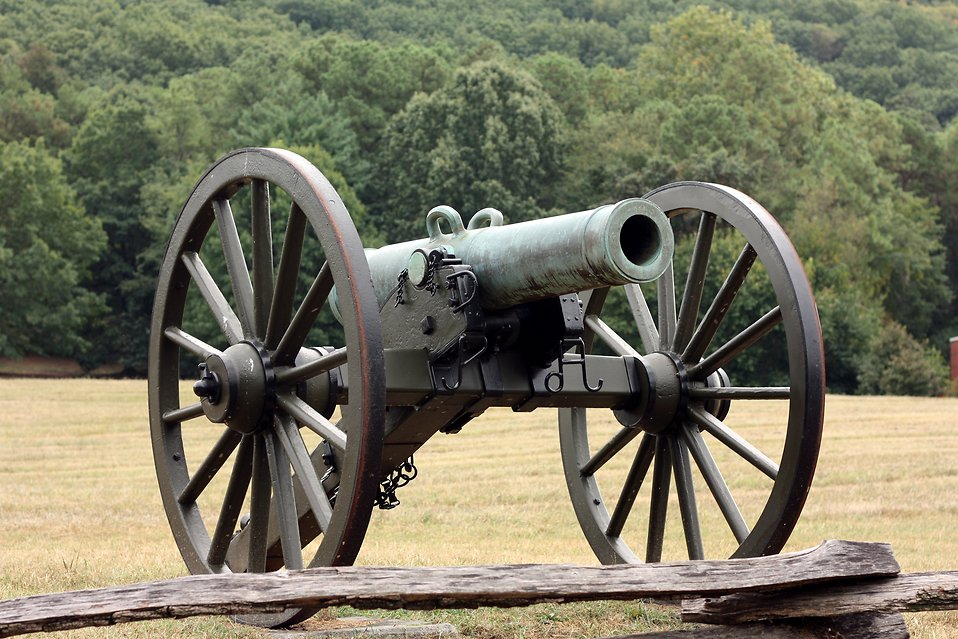
\includegraphics[width=8cm]{Pictures/Cannon.jpg}
    \caption{A cannon from 1864}
    \label{fig:cn}
\end{figure}

\begin{center}
    A \textbf{cannon} is a large-caliber gun classified as a type of artillery, which usually launches a \underline{projectile} using explosive chemical propellant. \textit{Gunpowder ("black powder")} was the primary propellant before the invention of smokeless powder during the late 19th century. Cannons vary in gauge, effective range, mobility, rate of fire, angle of fire and firepower; different forms of cannon combine and balance these attributes in varying degrees, depending on their intended use on the battlefield. A cannon is a type of heavy artillery weapon.
    The earliest known \textbf{depiction} of cannons appeared in Song dynasty China as early as the 12th century (Table: \ref{tab:cn}); however, solid archaeological and documentary evidence of cannons do not appear until the 13th century.
\end{center}

\begin{table}[h]
\begin{tabular}{ll}
\multicolumn{2}{l}{The earliest descriptions of cannons} \\
East Asia                    & 1128               \\
Western Europe               & 1322               \\
Islamic world                & 1274               \\
Eastern Europe               & 1382              
\end{tabular}
\label{tab:cn}
\end{table}

One can calculate the exact \textbf{distance} and \textbf{time} of flight of the launched projectile knowing only the initial velocity and the angle of the cannon shot. 
\[d = \frac{v^2sin(2\alpha)}{g}\]
\[t = \frac{2vsin(\alpha)}{g}\]

That is however, assuming no air resistance, no difference of height levels and no earth curvature.

\textbf{The main elements of the cannon include:}
\begin{itemize}
    \item neck
    \item muzzle
    \item chase girdle
    \item rimbases
    \item breech
    \item base ring
    \item knob
    \item fillet
\end{itemize}

\textbf{Artillery gets separated into different categories:}\par
\begin{enumerate}
    \item Infantry support guns
    \item Mountain guns
    \item Field guns
    \item Howitzers
    \item Gun-howitzers
    \item Mortars
    \item Gun-mortars
    \item Tank guns
    \item Anti-tank artillery
    \item Anti-tank guns
    \item Anti-aircraft artillery
\end{enumerate}

